\chapter{評価}
\begin{large}
\begin{quote}
本章では本システムの評価を行い,
結果について考察する.
\end{quote}
\end{large}
\clearpage

\section{評価方針}
本節では,本システムが
\ref{sec:requirements}で示した機能要件を満たしているかどうかを
実験を行うことで評価する.
具体的な方法について以下に述べる.


\begin{enumerate}
\item{リアルタイム性}\\
本研究は環境モニタリングやターゲットトラッキングのような
無線センサネットワークにおけるアプリケーションを対象としているため,
イベントモデルである拡張する前のContikiと本システムを比較し,
リアルタイムイベント発生から実行までの時間を評価する.
\newline
\item{消費電力}\\
本システムではリアルタイム処理が必要なイベントが発生しない場合には,
イベントモデルを採用している.
本要件が満たされているかどうかを確認するために,
純粋なスレッドモデルであるNano-RK上で同様の動作をするアプリケーションを実行し,
その際に消費される電力について評価を行う.
\end{enumerate}




%一般的なイベント駆動型のオペレーティングシステムでは,
%タスクは実行待ち状態になった順に実行されるため,
%重要なタスクが実行されず,
%そのタスク実行時にはその価値がなくなってしまうこともあるだろう.
%リアルタイム処理をサポートすれば,
%重要なタスクから順に処理を実行していくため,
%このように重要なタスクを未処理のまま終えてしまうような
%事態を未然に防ぐことができる.
%
%リアルタイム処理をサポートすることにより,
%低消費電力での運用も実現可能となる.
%リアルタイムタスクを効率的に処理可能なオペレーティングシステムと,
%効率の悪いオペレーティングシステムを比較した場合,
%前者の方が同じ精度のサービスを実現する場合に
%低いクロックで動作することができる.
%また,センサノード上では無線やセンサなどの
%周辺デバイスは必要のないときにスリープされることで消費電力を抑えている.
%このとき,リアルタイムタスクが処理可能ならば,
%素早く周辺デバイスのオンとオフを
%切り替えることができるようになるため,
%低消費電力を維持することが期待される.
%さらに,リアルタイム処理をサポートすることで,
%効率的に無線資源を利用し,
%無線通信に伴う電力を削減することができるだろう.



\section{リアルタイム性における評価}
\subsection{導入}
タスクの総数を一定にした場合と
タスクの総数を変化させる場合についてそれぞれ,
イベント発生の頻度を変化させながら,
リアルタイムイベントが発生してから
対象となるタスクが実行されるまでの時間(Latency)を評価する.
イベント発生の頻度を変化させるために,
Contikiにおけるイベントタイマーによってセットされる値を変化させる.
イベントタイマーは,
タイマーと現在時刻を比較し,
発火時刻をすぎている場合,
タスクをキューへと加える.
タイマーを実行するタスクは他のタスクと同じ優先度で周期的に実行される.
%イベント発生の頻度に関しては,
%1秒あたりの
%システムクロックによって生成される一定のテンポ(tick)数を
%CLOCK\_CONF\_SECONDとし,
%イベント発生の時刻をこのCLOCK\_CONF\_SECONDを
%具体的に,基準となる値(CLOCK\_CONF\_SECOND)を用いて変化させていく.
また,システムの安定性を評価するために,
累積確率密度関数(Cumulative Distribution Function)
を評価に取り入れ,
その結果について\ref{sec:rt_discussion}にて考察する.



\subsection{評価環境}
本評価ではContikiのために設計された仮想マシン上の
シミュレータCooja\cite{osterlind2006cross}を利用する.
仮想マシンの詳細を表\ref{tab:instant_contiki}に記す.
また\ref{sec:implement_env}で示したように,
本実験では対象とするノードとしてMicaZ\cite{Hill:2002:MWP:623308.624560}
を利用する.
%を利用し,タスクの総数とイベント発生の頻度を変化させ,
%それぞれについてリアルタイムイベントが発生してから,
%対象となるタスクが実行されるまでの時間(Latency)を
%評価する.

\begin{table}[htbp]
  \centering
  \caption{評価環境}
  \begin{tabular}{|l||c|} \hline
  	項目	 & 環境 \\ \hline \hline
	オペレーティングシステム & Ubuntu 12.04 \\ \hline
	メモリ & 1024 MB \\ \hline
  \end{tabular}
  \label{tab:instant_contiki}
\end{table}






\subsection{実験結果}
%本評価項目における結果について示す.
%イベント発生の頻度に関しては,
%1秒あたりの
%システムクロックによって生成される一定のテンポ(tick)数を
%CLOCK\_CONF\_SECONDとし,
%イベント発生の時刻をこのCLOCK\_CONF\_SECONDを
タスクの総数を一定にした場合と
タスクの総数を変化させる場合についてそれぞれ,
%イベント発生の頻度を変化させながら,
実験によって得られた結果を示す.
ここで示すContikiは拡張前のContikiを,
D-Switchは拡張された後のContikiを示している.

\subsubsection{タスクの総数を固定した場合}

\vspace{0.5em}タスクの総数を固定し,
イベントの発生頻度を増やしながら実験を300秒ずつ,3回行った.

\begin{enumerate}
\item{実験1}\\
表\ref{tab:latency1},図\ref{fig:latency1}
からわかるように,
D-SwitchとContikiを比較してみると,
最小値,中央値の値に差異は見られない.
しかしながら,
ContikiにおけるLatencyの最大値が
163msを記録することが数回あったため,
平均値,標準偏差ともにD-Switchを上回る結果となった.
また図\ref{fig:cdf1}より,
Contikiでは最小値を記録した回数が
D-Switchよりも多いが,
D-SwitchではLatencyが81ms以下となる場合が
98\%を占めているため,
D-Switchの方が安定して低いLatencyを維持することに成功している.
\newline
\item{実験2}\\
表\ref{tab:latency2},図\ref{fig:latency2}より
実験1と同様にLatencyを比較したところ,
最小値,中央値の値に差異はなく,
最大値は実験1で得られた値に等しい.
しかしながら,
実験1と比較して,ContikiにおけるLatencyが最大となる
場合が多く,平均値,標準偏差の値が増加した.
図\ref{fig:cdf2}により得られた
累積密度確率関数の結果も
図\ref{fig:cdf1}と類似している.
\newline
\item{実験3}\\
表\ref{tab:latency3},図\ref{fig:latency3}が示すとおり,
最小値はContikiがD-Switchを下回ったが,
最大値はContikiがD-Switchを上回る245msを記録しているため,
ContikiにおけるLatencyの
平均値,標準偏差がそれぞれD-Switchを上回る結果となった.
%上記の実験と比較して,
%D-Switchは平均値,標準偏差ともに大きな変化は見られないが,
%実験2と比較したところ,
さらに図\ref{fig:cdf3}より,
D-Switchでは94\%が81msのLatencyでリアルタイムタスクの実行を
行うことができており,
安定性においてD-Switchの優位性を示している.
\end{enumerate}


\begin{table}[htbp]
  \centering
  \caption{実験結果1}
  \begin{tabular}{|c||c|c|c|c|c|} \hline
    \backslashbox{}{} & 最小値 & 最大値 & 中央値 & 平均値 & 標準偏差 \\ \hline \hline
    D-Switch & 80 & 82 & 81 & 81 & 0.17 \\ \hline
    Contiki & 80 & 163 & 81 & 97.97 & 33.39 \\ \hline
  \end{tabular}
  \label{tab:latency1}
\end{table}

\begin{figure}[htbp]
 \begin{center}
  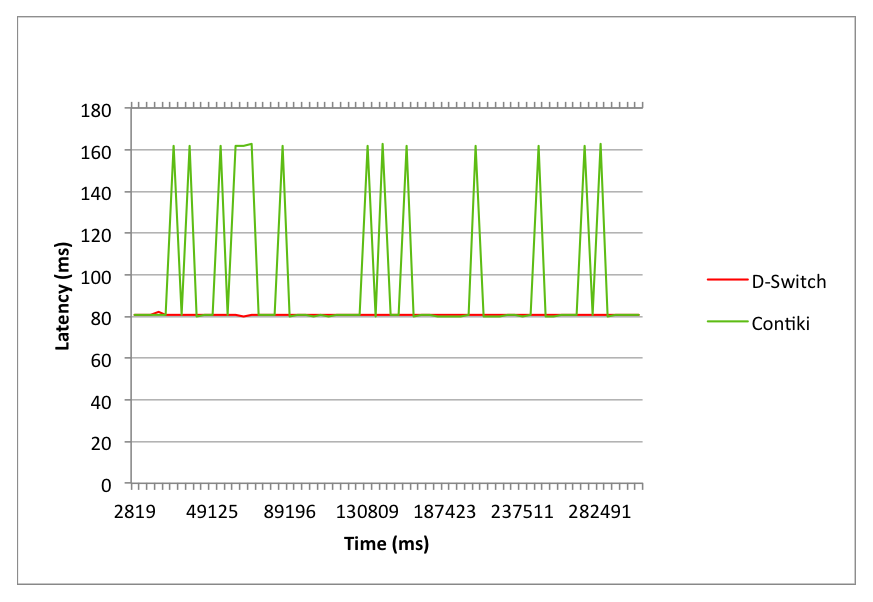
\includegraphics[width=120mm]{./images/latency1.eps}
 \end{center}
 \caption{実験結果1}
 \label{fig:latency1}
\end{figure}

\begin{figure}[htbp]
 \begin{center}
  \includegraphics[width=120mm]{./images/cdf1.eps}
 \end{center}
 \caption{実験結果1}
 \label{fig:cdf1}
\end{figure}


\begin{table}[htbp]
  \centering
  \caption{実験結果2}
  \begin{tabular}{|c||c|c|c|c|c|} \hline
    \backslashbox{}{} & 最小値 & 最大値 & 中央値 & 平均値 & 標準偏差 \\ \hline \hline
    D-Switch & 80 & 82 & 81 & 81.02 & 0.19 \\ \hline
    Contiki & 80 & 163 & 81 & 108.37 & 38.49 \\ \hline
  \end{tabular}
  \label{tab:latency2}
\end{table}

\begin{figure}[htbp]
 \begin{center}
  \includegraphics[width=120mm]{./images/latency2.eps}
 \end{center}
 \caption{実験結果2}
 \label{fig:latency2}
\end{figure}

\begin{figure}[htbp]
 \begin{center}
  \includegraphics[width=120mm]{./images/cdf2.eps}
 \end{center}
 \caption{実験結果2}
 \label{fig:cdf2}
\end{figure}


\begin{table}[htbp]
  \centering
  \caption{実験結果3}
  \begin{tabular}{|c||c|c|c|c|c|} \hline
    \backslashbox{}{} & 最小値 & 最大値 & 中央値 & 平均値 & 標準偏差 \\ \hline \hline
    D-Switch & 81 & 82 & 81 & 81.02 & 0.24 \\ \hline
    Contiki & 80 & 245 & 81 & 98.36 & 49.61 \\ \hline
  \end{tabular}
  \label{tab:latency3}
\end{table}

\begin{figure}[htbp]
 \begin{center}
  \includegraphics[width=120mm]{./images/latency3.eps}
 \end{center}
 \caption{実験結果3}
 \label{fig:latency3}
\end{figure}

\begin{figure}[htbp]
 \begin{center}
  \includegraphics[width=120mm]{./images/cdf3.eps}
 \end{center}
 \caption{実験結果3}
 \label{fig:cdf3}
\end{figure}



\subsubsection{タスクの総数を変化させた場合}

\vspace{0.5em}タスクの総数を増やしながら
実験を300秒ずつ,2回行った.

\begin{enumerate}
\item{実験4}\\
表\ref{tab:latency4},図\ref{fig:latency4}が示すとおり,
ContikiではLatencyの最小値が80msを記録し,
両者における最小値となったが,
D-Switchでは観測されたすべての値が81msを記録しており,
標準偏差0を示したことや,
100\%が81msのLatencyで実行されていること
(図\ref{fig:cdf4})からも,
本システムの安定性を裏付ける結果となった.
\newline
\item{実験5}\\
表\ref{tab:latency5},図\ref{fig:latency5}より,
Contikiにおける最大値,平均値,標準偏差は
全実験中最大の値となった.
それに対して,D-Switchは
図\ref{fig:cdf5}にも示されるように,
97\%が81ms以内にリアルタイムタスクの実行を許可されている.
\end{enumerate}



\begin{table}[htbp]
  \centering
  \caption{実験結果4}
  \begin{tabular}{|c||c|c|c|c|c|} \hline
    \backslashbox{}{} & 最小値 & 最大値 & 中央値 & 平均値 & 標準偏差 \\ \hline \hline
    D-Switch & 81 & 81 & 81 & 81 & 0 \\ \hline
    Contiki & 80 & 326 & 81 & 102 & 48.52 \\ \hline
  \end{tabular}
  \label{tab:latency4}
\end{table}

\begin{figure}[htbp]
 \begin{center}
  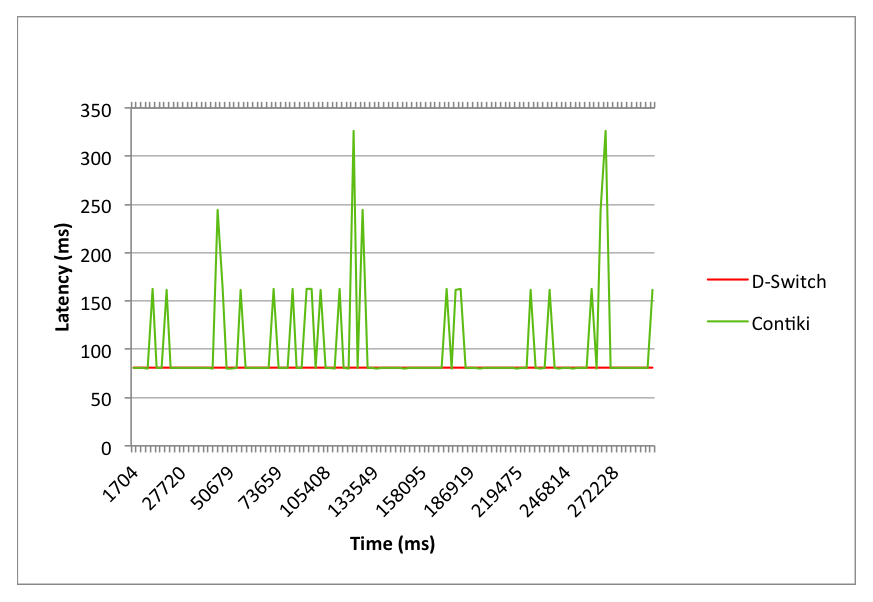
\includegraphics[width=120mm]{./images/latency4.eps}
 \end{center}
 \caption{実験結果4}
 \label{fig:latency4}
\end{figure}

\begin{figure}[htbp]
 \begin{center}
  \includegraphics[width=120mm]{./images/cdf4.eps}
 \end{center}
 \caption{実験結果4}
 \label{fig:cdf4}
\end{figure}



\begin{table}[htbp]
  \centering
  \caption{実験結果5}
  \begin{tabular}{|c||c|c|c|c|c|} \hline
    \backslashbox{}{} & 最小値 & 最大値 & 中央値 & 平均値 & 標準偏差 \\ \hline \hline
    D-Switch & 80 & 82 & 81 & 81.02 & 0.21 \\ \hline
    Contiki & 80 & 327 & 81 & 121.26 & 63.95 \\ \hline
  \end{tabular}
  \label{tab:latency5}
\end{table}

\begin{figure}[htbp]
 \begin{center}
  \includegraphics[width=120mm]{./images/latency5.eps}
 \end{center}
 \caption{実験結果5}
 \label{fig:latency5}
\end{figure}

\begin{figure}[htbp]
 \begin{center}
  \includegraphics[width=120mm]{./images/cdf5.eps}
 \end{center}
 \caption{実験結果5}
 \label{fig:cdf5}
\end{figure}


\subsection{考察}\label{sec:rt_discussion}
ここでは,リアルタイムイベントが発生してから
タスクが実行されるまでの時間について考察を行う.
実験1から実験3からわかるようにイベントの発生頻度が
増加した場合,
ContikiではLatencyが増加することが伺える.
同様に実験4から実験5のようなタスクの総数が増加した場合にも,
ContikiにおけるLatencyは増加する傾向にある.

\ref{sec:asynchronous_event},\ref{sec:problems}
で示したように,
Contikiでは発生したイベントは
FIFOの要領でポストされていくため,
イベントが発生された際に
キューにすでに実行待ちのイベントが挿入されていた場合,
実行される時間が遅くなってしまう.
それに対して,
D-Switchでは,リアルタイムイベントが発行された際には,
実行中のタスクがあった場合でも,
そのタスクの実行を一時中断して,
リアルタイムタスクの実行を行うことができるため,
Latencyを低く維持することを可能にしている.


\section{消費電力における評価}

\subsection{評価環境}


\subsection{実験結果}


\subsection{考察}



\section{まとめ}
%本章では,まず,本研究に評価方針,実験環境を述べた.次に,実験環境内における実験への影響を調査するため,それぞれのリージョンからICMPにおける,Message Requestを送信し,リプライが返されるまでの時間(RTT)を計測した.その結果,RTTは0.400ms以内であり,十分に無視できることを述べた.次いで,保存ピア探索における計算コスト,データの保存に要する時間,データの取得に要する時間の観点から評価を行った.その結果から,考察を行い,理論値と実際の値に齟齬が存在することを明らかにし,その違いは,T-Ringにおいて,保存や取得の対象となるデータの時間情報の取得を行う際に要する時間により生じていることに言及した.
